%%%%%%%%%%%%%%%%%%%%%%%%%%%%%%%%%%%%%%%%%
% Beamer Presentation
% LaTeX Template
% Version 1.0 (10/11/12)
%
% This template has been downloaded from:
% http://www.LaTeXTemplates.com
%
% License:
% CC BY-NC-SA 3.0 (http://creativecommons.org/licenses/by-nc-sa/3.0/)
%
%%%%%%%%%%%%%%%%%%%%%%%%%%%%%%%%%%%%%%%%%

%----------------------------------------------------------------------------------------
%	PACKAGES AND THEMES
%----------------------------------------------------------------------------------------

\documentclass{beamer}

\mode<presentation> {
\usetheme{Madrid}
\usefonttheme{serif} 
\setbeamertemplate{navigation symbols}{} % To remove the navigation symbols from the 
}
\usepackage{lmodern}  
\usepackage{graphicx} % Allows including images
\usepackage{booktabs} % Allows the use of \toprule, \midrule and \bottomrule in tables
\usepackage[T1]{fontenc}
\usepackage[utf8]{inputenc}
\usepackage{amsmath}
\usepackage{caption} 
\usepackage{color}
\usepackage[czech]{babel}
\usepackage{lmodern}  
\usepackage{rotating}
\usepackage{scrextend}
\usepackage{pifont}
\usepackage{hyperref}
\usepackage{bm}
\usepackage{tikz}
\usetikzlibrary{arrows,positioning}
\usetikzlibrary{calc}
%
\newcommand*\circled[1]{\tikz[baseline=(char.base)]{
    \node[shape=circle,draw=red,inner sep=2pt] (char) {#1};}}
%
\newcommand*\circledd[1]{\tikz[baseline=(char.base)]{
    \node[shape=circle,draw=ProcessBlue, dashed, inner sep=2pt] (char) {#1};}}
%
\newcommand{\mytikzmark}[2]{%
  \tikz[remember picture,inner sep=0pt,outer sep=0pt,baseline,anchor=base] 
    \node (#1) {\ensuremath{#2}};}
%
%
\newcommand*{\boxcolor}{Red}
\makeatletter
\renewcommand{\boxed}[1]{\textcolor{\boxcolor}{%
\tikz[baseline={([yshift=-1ex]current bounding box.center)}] \node [rectangle,semithick, minimum width=1ex,draw, dashed] {\normalcolor\m@th$\displaystyle#1$};}}
 \makeatother
%
%------------------------------
%	TITLE PAGE
\title[Block 6]{Praktikum z ekonometrie} 
\author{VŠE Praha} 
\institute[4EK417] 
{
% Your institution for the title page
\medskip
\textit{Tomáš Formánek} % Your email address
}
\date{} % Date, can be changed to a custom date
%------------------------------
\begin{document}
\begin{frame}
\titlepage % Print the title page as the first slide
\end{frame}
%------------------------------
\begin{frame}
\frametitle{Block 6 – Treatment effects – Outline
} 
\tableofcontents 
\end{frame}
%------------------------------
\section{Treatment effects: Introduction}
\begin{frame}{Treatment effects: Introduction}
\begin{itemize}
    \item \textbf{Treatment effect analysis:} to evaluate the impact of intervention (treatment) on some \textbf{outcome} of interest.
    \bigskip
    \item Response to treatment is evaluated relative to a benchmark:  \\no treatment (control) or different treatment. 
    \bigskip
    \item Analysis of treatment effect is typically based on regression models, with outcome as the dependent variable.
    \bigskip
    \item Treatment effect analysis is generally based on the framework of Rubin's causal model. 
\end{itemize}
\end{frame}
%------------------------------
\begin{frame}{Treatment effects: Introduction}
\textbf{Examples}\\ \medskip
\begin{itemize}
    \item Wage effect of enrollment in a skill-training program.
    \medskip
    \item Health effects (speed of recovery), if new drug / medical procedure is used.
    \medskip
    \item Student performance upon being educated in small classes as opposed to large classes (being in a small class is the treatment). 
\end{itemize}
\bigskip
\textbf{Key topics of the analysis:}\\
Treatment participation: random assignment or self selection?\\
Treatment effects: actual effects or influence by confounding factors?\\
\bigskip
\textbf{Multiple treatments:} If treatment varies in intensity or type. Same principle of analysis, the choice of benchmark is more flexible.
\end{frame}
%------------------------------
% Define box and box title style
\tikzstyle{mybox} = [draw=blue!35, fill=white, very thick,
    rectangle, rounded corners, inner sep=1pt, inner ysep=10pt]
\tikzstyle{fancytitle} =[fill=blue!35, text=black]
%---------------------------------
\begin{frame}{Treatment effects: Basic notation \& terminology}
\begin{itemize}
    \item Every $i$th individual in a population has a potential outcome $y_i$ and can be exposed to treatment $C_i=\{0;1\}$. 
    \medskip
    \item $y_{i1} = y_i | (C_i = 1) $ for the treated, and \\
    $y_{i0} = y_i | (C_i = 0)$ for the non-treated.
    \medskip
    \item Average treatment effect (averaged across population):
    $$\textnormal{ATE} = E \left[ y_{i1}-y_{i0}\right],$$
    and the $i$th observation only exist in one of the two states.
    \medskip
    \item \textbf{Average treatment effect of the treated} is more of interest:
    $$\textnormal{ATET} = E \left[ y_{i1}-y_{i0} | C_i = 1\right],$$
    and the second term $y_{i0}$ is a missing counterfactual. 
    \medskip
    \item Individuals will only exist in one state: treated/untreated. Multiple assumptions apply for ATE/ATET estimation.
\end{itemize}  
\end{frame}
%------------------------------
\begin{frame}{Treatment effects: Study \& data types}
\textbf{Types of studies and data used for TE analysis}:\\
\begin{itemize}
    \item Scientific experiments under randomisation: assignment into treated and control groups is random. Relatively rare in socio-economic studies. 
    \medskip
    \item Observational studies (natural experiments, quasi-experiments): assignment into treatment and control group is not random. \\ \medskip
\end{itemize}
\bigskip
\textbf{Main problems of TE analysis:}
\begin{itemize}
    \item \textbf{Endogeneity of treatment} and self-selection bias: if treatment participation is optional, individuals who choose to participate may be systematically different from non-participants.
    \medskip
    \item \textbf{Missing counterfactual:}  Individuals always measured as either treated or untreated, we cannot observe both $y_{i1}$ and $y_{i0}$.
\end{itemize}
    

\end{frame}
%---------------------------------
\begin{frame}{Treatment effects: Study \& data types}
\begin{tikzpicture}
\node [mybox] (box){%
\begin{minipage}{0.50\textwidth}
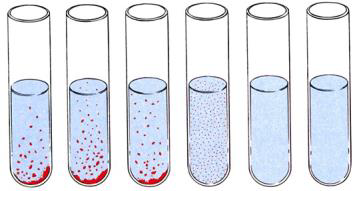
\includegraphics[width=\textwidth, height=2.89cm]{./IMG/Obrazek1}
\begin{itemize}
\scriptsize
\item Test tubes identical except for catalyst
\item Measure: Effect at different catalyst volumes (reaction speed, product volume, \dots)
\item Perform the experiment $n$-times
\item Control for other factors (heat, \dots)
\item Estimate average effects \& standard errors
\end{itemize}
\end{minipage}
};
\node[fancytitle, right=5pt,  rounded corners] at (box.north west) {\scriptsize Scientific experiment};
\end{tikzpicture}%
\begin{tikzpicture}
\node [mybox] (box){%
\begin{minipage}{0.50\textwidth}
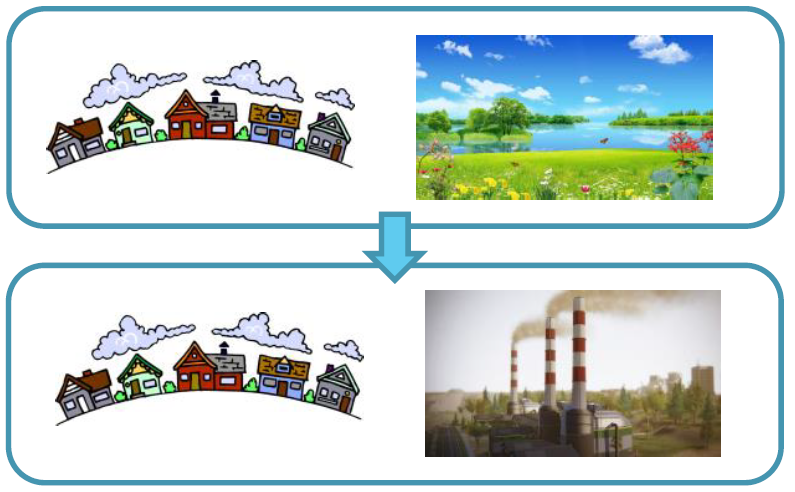
\includegraphics[width=\textwidth]{./IMG/Obrazek2}
\begin{itemize}
\scriptsize
\item Garbage incinerator is built in one given
suburban area over time
\item How do we estimate the effect on
individual house-prices?
\item Identical control group does not exist…
\item Different estimators exist -- multiple
assumptions apply!
\end{itemize}
\end{minipage}
};
\node[fancytitle, right=5pt,  rounded corners] at (box.north west) {\scriptsize Natural experiment (quasi-experiment)};
\end{tikzpicture}%
\end{frame}
%---------------------------------
\begin{frame}{Treatment effects: Three main approaches to analysis}
Types of analysis, key assumptions \& requirements:\\
\bigskip
\begin{itemize}
    \item \textbf{Differences in differences (DiD) estimator}\\
        \begin{itemize}
            \item Independence of treatment on the outcome at the base ($y_{i0}$), \\i.e. treatment assignment exogenous/random
            \item Parallel trends assumed
        \end{itemize}
    \bigskip
    \item \textbf{Propensity score matching (PSM):}
        \begin{itemize}
            \item Unconfoundedness (treatment assignment as good as random \\after accounting for covariates)
            \item Common support (for the treated and untreated)
            \item Large sample 
        \end{itemize}
    \bigskip
    \item \textbf{Regression discontinuity design (RDD):}
        \begin{itemize}
            \item Assignment variable \& assignment threshold exist
            \item Local randomization assumed
        \end{itemize}
\end{itemize}
\end{frame}
%---------------------------------
\begin{frame}{Treatment effects: Unconfoundedness}
\begin{center}
\begin{tikzpicture}[
    box/.style={rectangle, draw, minimum size=0.6cm},
    arrow/.style={thick,->,>=stealth}
]
\node[box] (box4) at (-3,0) {Exposure};
\node[box] (box5) at (3,0) {Outcome};
\draw [dotted, ->] (box4) -- (box5) node[midway, above, red] {Treatment effect};
\end{tikzpicture}
\end{center}
%
\begin{center}
\begin{tikzpicture}[
    box/.style={rectangle, draw, minimum size=0.6cm},
    arrow/.style={thick,->,>=stealth}
]
\node[box] (box1) at (0,0) {Confounder};
\node[box] (box2) at (-3,-0.6) {Exposure};
\node[box] (box3) at (3,-0.6) {Outcome};
\draw[arrow] (box1) -> (box2);
\draw[arrow] (box1) -> (box3);
\draw [dotted, ->] (box2) -- (box3) node[midway, red] {$\times$};
\end{tikzpicture}
\end{center}
Often: combination of actual TE \& confounding factor influence.\\
\bigskip
\small  
\textbf{Example:} Company has two types of trucks, A and B (using the new A-Truck is the treatment). We want to compare fuel efficiency (outcome). Using MPG, we find A-Trucks are more efficient. However, A-Trucks often drive on highways, while B-Trucks are mostly in the city. This route difference is a confounding variable, making our results unreliable as highway driving is generally more fuel-efficient. \\
\smallskip
To improve the study, we could randomize truck assignments for equal city and highway driving, introduce city driving as another independent variable to a model, or segment the study into city and highway driving comparisons.
\end{frame}
%---------------------------------
\begin{frame}{Treatment effects: Unconfoundedness}
\textbf{Unconfoundedness} states that the potential outcomes are independent of the treatment assignment, conditional on a set of observed covariates. Once we control for these covariates, the treatment \emph{assignment} does not provide any additional information about the \emph{potential} outcomes:
$$
(y_0, y_1) \perp  \textit{Tr} ~|~ \bm{X},
$$
- $(y_0)$ and $(y_1)$ are the potential outcomes under control and treatment,\\
- $\textit{Tr}$ is the treatment assignment (dummy variable), \\
- $\bm{X}$ is the set of observed covariates. \\
\bigskip
\textbf{Independence of treatment on the outcome at the base (for the untreated)} is a stronger assumption. Here, the potential outcome under control is independent of the treatment assignment, even without conditioning on covariates:
$$
y_0 \perp \textit{Tr}
$$
\end{frame}
%---------------------------------
\begin{frame}{Treatment effects: Unconfoundedness}
\textbf{Unconfoundedness} assumption allows for the possibility that treatment assignment might be related to the potential outcomes through the observed covariates. Once we control for these covariates, the treatment assignment is assumed to be as good as random. \\
\bigskip
\textbf{Independence of treatment on the outcome} assumption requires the treatment assignment to be as good as random without conditioning on any covariates. This is a stronger assumption and is less likely to hold in real-world situations.
\end{frame}
%---------------------------------
\begin{frame}{Treatment effects: Unconfoundedness \& \texttt{do()} notation}
\small 
$$P(Y|\texttt{do}(X)) = P(Y)$$ 
LHS can be red as: ``the probability of $Y,$ given that you do  $X$''. The expression above describes the case where $Y$ is independent of doing $X$.\\
\bigskip
Say, we have an outcome $y$, a dummy treatment variable $\textit{Tr}$ and potential counfounding variable $z$ that influences both $y$ and $\textit{Tr}$. If unconfoundedness holds, the following equation holds
$$P(y | \texttt{do}(\textit{Tr})) = P(y|\textit{Tr})$$
for all values $\textit{Tr}$ and $y$, where $P(y|\textit{Tr})$ is the conditional probability. This equality states that $\textit{Tr}$ and $y$ are not confounded whenever the observationally witnessed association between them is the same as the association that would be measured in a controlled experiment, with $\textit{Tr}$ randomized. Otherwise, we have to account for the confounding factor $z$:
$$P(y | \texttt{do}(\textit{Tr})) = \sum_z P(y|\textit{Tr},z)P(z). $$
\centering
\url{https://en.wikipedia.org/wiki/Confounding}
\end{frame}
%---------------------------------
\begin{frame}{Treatment effects analysis}
\textbf{Estimation approaches for TE analysis:}\\
\bigskip
\begin{enumerate}
    \item Differences in differences (DiD)
    \bigskip
    \item Propensity score matching (PSM):
    \bigskip
    \item Regression discontinuity design (RDD):
\end{enumerate}
\end{frame}
%---------------------------------
\section{Differences in differences (DiD) estimator}
\begin{frame}{DiD: Introduction \& example}
\vfill
{\footnotesize \textbf{Treatment: employee training for women returning from maternal leave\\ Outcome: wage effect}} \\
\medskip
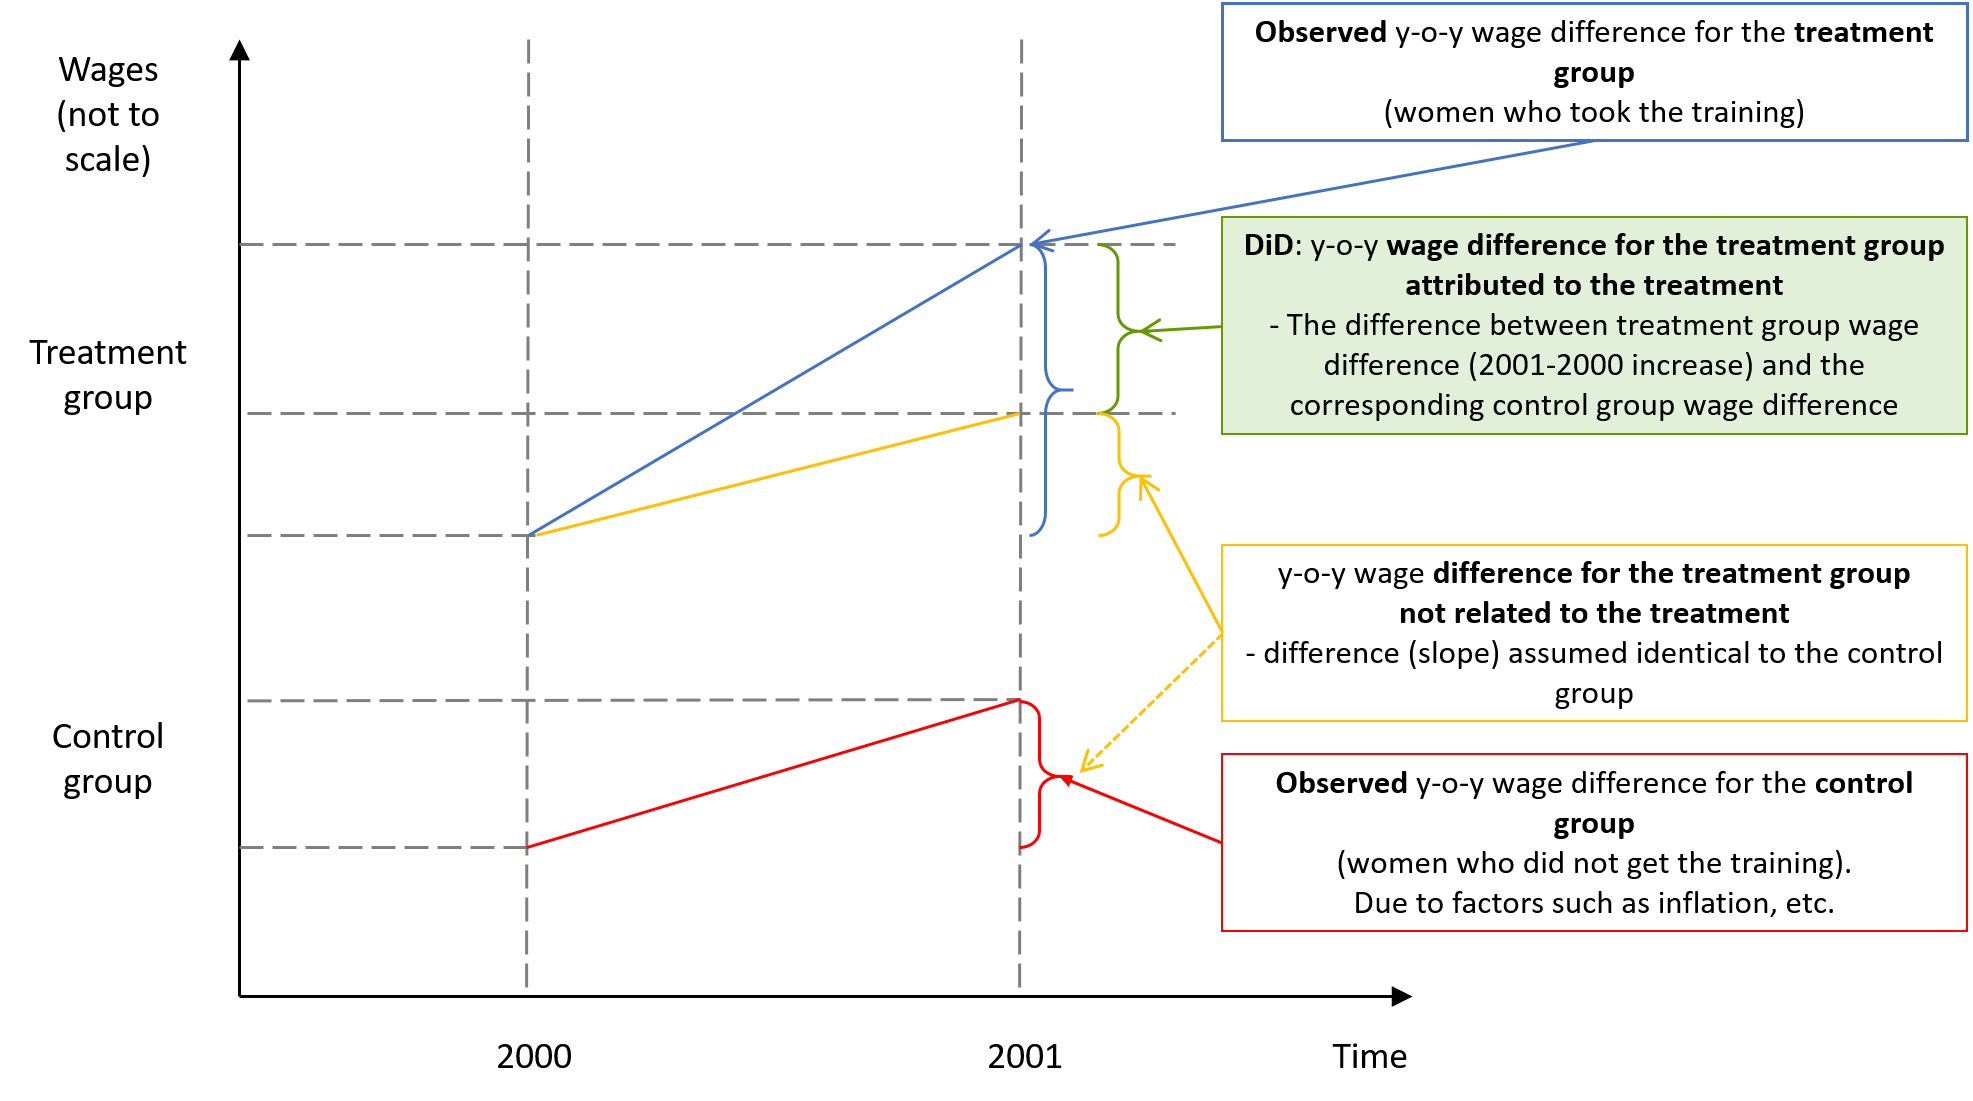
\includegraphics[width=\textwidth]{./IMG/Obrazek3}
\end{frame}
%---------------------------------
\begin{frame}{DiD estimator: Assumptions}
\begin{itemize}
    \item \emph{Exchangeability (parallel trends)}: in the absence of treatment, the average outcomes for the treated and control groups would follow the same trend over time.
    \item \emph{Positivity}: every individual (unit) has a positive probability of receiving the treatment.
    \item \emph{Stable unit treatment value assumption (SUTVA)}: the potential outcomes for any individual do not depend on the treatment assignment of the other individuals.
    \item \emph{No spillover effects}: the treatment of one individual does not affect the outcome of another individual.
    \item \emph{Treatment unrelated to outcome at baseline}: the allocation of treatment is not determined by the outcome. 
    \item \emph{Stable composition of treatment and control groups}: applies to repeated treatments/interventions.
\end{itemize}
\end{frame}
%---------------------------------
\begin{frame}{DiD: Model motivation}
\small
With cross-sectional data and \textbf{exogenous}  treatment variable $D = \{0;1\}$, \\we can formulate (estimate, interpret) a regression model such as:
$$
y_i = \bm{x}_i^{\prime}\bm{\beta} + \delta D_i + \varepsilon_i.
$$\\
\medskip
\textbf{DiD estimator} refers to panel-based (or using pooled CS data) analysis, based on two dummy variables and their interaction: $T$ differentiates between two time periods (before/after treatment) and $D$ distinguishes the two groups (treatment/control):
$$y_{it}=\beta_0 + \beta_1 D_i + \beta_2 T_t + \delta_1 (D_i T_t) + \bm{x}_i^{\prime}\bm{\beta} + \varepsilon_{it}.$$

\end{frame}
%---------------------------------
\begin{frame}{DiD estimator: Model description} 
\medskip 
$$y_{it}=\beta_0 + \beta_1 D_i + \beta_2 T_t + \delta_1 (D_i T_t) + \varepsilon_{it},$$
where:
\begin{itemize}
\item $i=1, \dots, N;~~t=1,2$. \\
\item[$T_t$] is a time dummy, $T_1=0$ is the first (pre-treatment) period and \\$T_2 = 1$ is the second period (post treatment),
\item[$D_i$] is a treatment dummy, $D_i=1$ for the treated,
\item[$D_i T_t$] is an interaction element, i.e. $(D_i\! \cdot \! T_t)$,
\item[$\delta_1$] is the DiD estimator (coefficient). 
\end{itemize}
\bigskip
For simplicity, the term $\bm{x}_{it}^{\prime}\bm{\beta}$ is removed here. Note that adding $\bm{x}_{it}^{\prime}\bm{\beta}$ back to the model doesn't change the general interpretation of $\delta_1$.
\end{frame}
%---------------------------------
\begin{frame}{DiD estimator: Interpretation of the DiD $\delta_1$ coefficient}
$$y_{it}=\beta_0 + \beta_1 D_i + \beta_2 T_t + \delta_1 (D_i T_t) + \varepsilon_{it}$$\\
\bigskip
\footnotesize
\begin{table}
\captionsetup{labelformat=empty}
\centering
\caption{Table: Illustration of the DiD estimator}\label{Tab1}
\begin{tabular}{|l|c|c|c|}
\hline
\multicolumn{1}{|c|}{$E(y_{it} | D_i, T_t)$} & Before $(t = 1)$    & After $(t=2)$                             & After -- Before        \\ \hline
Control $(D_i=0)$                                    & $\beta_0$           & $\beta_0 + \delta_0$                      & $\delta_0$            \\ \hline
Treatment $(D_i=1)$                                  & $\beta_0 + \beta_1$ & $\beta_0 + \delta_0 + \beta_1 + \delta_1$ & $\delta_0 + \delta_1$ \\ \hline
Treatment -- Control                        & $\beta_1$           & $\beta_1 + \delta_1$                      & \circled{$\delta_1$}            \\ \hline
\end{tabular}
\end{table}

~\\
Again, if $\bm{x}_{it} \bm{\beta}$ is added back to the equation, interpretation of $\delta_1$ remains \\essentially unchanged.

\end{frame}
%---------------------------------
\begin{frame}{DiD estimator: Interpretation of the DiD $\delta_1$ coefficient}
$$y_{it}=\beta_0 + \beta_1 D_i + \beta_2 T_t + \delta_1 (D_i T_t) + \varepsilon_{it},$$\\
\bigskip
By rearranging an estimated model, we can express $\delta_1$ as follows:
\begin{align*}
\hat{\delta}_1 &= (\overline{y}_{Tr,\,t=2} - \overline{y}_{Co,\,t=2}) -  (\overline{y}_{Tr,\,t=1} - \overline{y}_{Co,\,t=1}), \\ ~& \\
& \hspace{0.5cm} \textnormal{which may be also rearranged as:} \\ ~& \\
&= (\overline{y}_{Tr,\,t=2} - \overline{y}_{Tr,\,t=1}) -  (\overline{y}_{Co,\,t=2} - \overline{y}_{\textit{Co},\,t=1}),
\end{align*}
where \\ \textit{Tr} subscript stands for treatment group, and \\ \textit{Co} subscript identifies the control group.
\end{frame}
%---------------------------------
\begin{frame}{DiD estimator: Example}
\footnotesize{What is the effect of building garbage incinerator on housing prices?}
\scriptsize
\begin{table}[]
\centering
\label{Tab21}
\begin{tabular}{lclcc}
\multicolumn{3}{l}{Dependent Variable: RPRICE}                                          &                      & \multicolumn{1}{l}{}      \\
\multicolumn{3}{l}{Included observations: 321}                                          &                      & \multicolumn{1}{l}{}      \\
                                &                      & \multicolumn{1}{c}{}           &                      & \multicolumn{1}{l}{}      \\
\multicolumn{1}{c}{Variable}    & Coefficient          & \multicolumn{1}{c}{Std. Error} & t-Statistic          & \multicolumn{1}{l}{Prob.} \\
                                
                                & \multicolumn{1}{l}{} &                                & \multicolumn{1}{l}{} & \multicolumn{1}{l}{}      \\
\multicolumn{1}{c}{(Intercept)}           & 82517.23             & \multicolumn{1}{c}{2726.910}   & 30.26034             & 0.0000                    \\
\multicolumn{1}{c}{Y81}         & 18790.29             & \multicolumn{1}{c}{4050.065}   & 4.639502             & 0.0000                    \\
\multicolumn{1}{c}{NEARINC}     & -18824.37            & \multicolumn{1}{c}{4875.322}   & -3.861154            & 0.0001                    \\
\multicolumn{1}{c}{Y81*NEARINC} & -11863.90            & \multicolumn{1}{c}{7456.646}   & -1.591051            & 0.1126                    \\
                                
                                & \multicolumn{1}{l}{} &                                & \multicolumn{1}{l}{} & \multicolumn{1}{l}{}      \\
R-squared                       & 0.173948             & \multicolumn{2}{l}{Mean dependent var}                & 83721.36                  \\
Adjusted R-squared              & 0.166131             & \multicolumn{2}{l}{S.D. dependent var}                & 33118.79                  \\
S.E. of regression              & 30242.90             & \multicolumn{2}{l}{Akaike info criterion}             & 23.48429                  \\
Sum squared resid               & 2.90E+11             & \multicolumn{2}{l}{Schwarz criterion}                 & 23.53129                  \\
Log likelihood                  & -3765.229            & \multicolumn{2}{l}{Hannan-Quinn criter.}              & 23.50306                  \\
F-statistic                     & 22.25107             & \multicolumn{2}{l}{Durbin-Watson stat}                & 1.557107                  \\
Prob(F-statistic)               & 0.000000             & \multicolumn{2}{l}{}                                  & \multicolumn{1}{l}{}     
\end{tabular}
\end{table}
\begin{tikzpicture}[<-,overlay,remember picture,inner sep=1.5pt,shorten <=0.2em,font=\footnotesize]
\tikzset{
    mynode/.style={rectangle,draw=blue, fill=blue!30, very thick, inner sep=.5em, minimum size=2em, text width=25em}
}
\node[mynode] at (7.8, 0.3) (Table){
\scriptsize{RPRICE - house price in real terms (USD) \\ 
$Y81$ – dummy variable for $1981$, \ ($t=1978,1981$),\\
~~$1978$ – before ``rumors''; $1981$ – incinerator operational \\
NEARINC – dummy for the treatment group}};
\end{tikzpicture}
\end{frame}
%---------------------------------
\begin{frame}{DiD estimator: selection bias}
\begin{block}{Selection bias (treatment effect vs. selection bias):}
\small
\textbf{Incinerator example:} Say, we have a “poor neighborhood” with relatively old and small houses and low house-prices. For complex reasons, it suffers from a representation deficit within the local city council (as compared to other “rich neighborhoods”) and is therefore more likely to get the incinerator. To address this problem, we would need variables to control for this factor.\\
\medskip
\textbf{Job training example:} For a natural experiment with job-training effects, we have voluntary participation. If more agile workers tend to participate more, we cannot assume treatment and control group are identical -- except for the treatment. Hence, besides of treatment effect, DiD would reflect latent ``propensity'' to participate.
\end{block}
\medskip 
DiD will be biased and inconsistent in both cases.
\end{frame}
%---------------------------------
\section{Propensity score matching}
\begin{frame}{Propensity score matching: Matching vs. PSM}
\centering
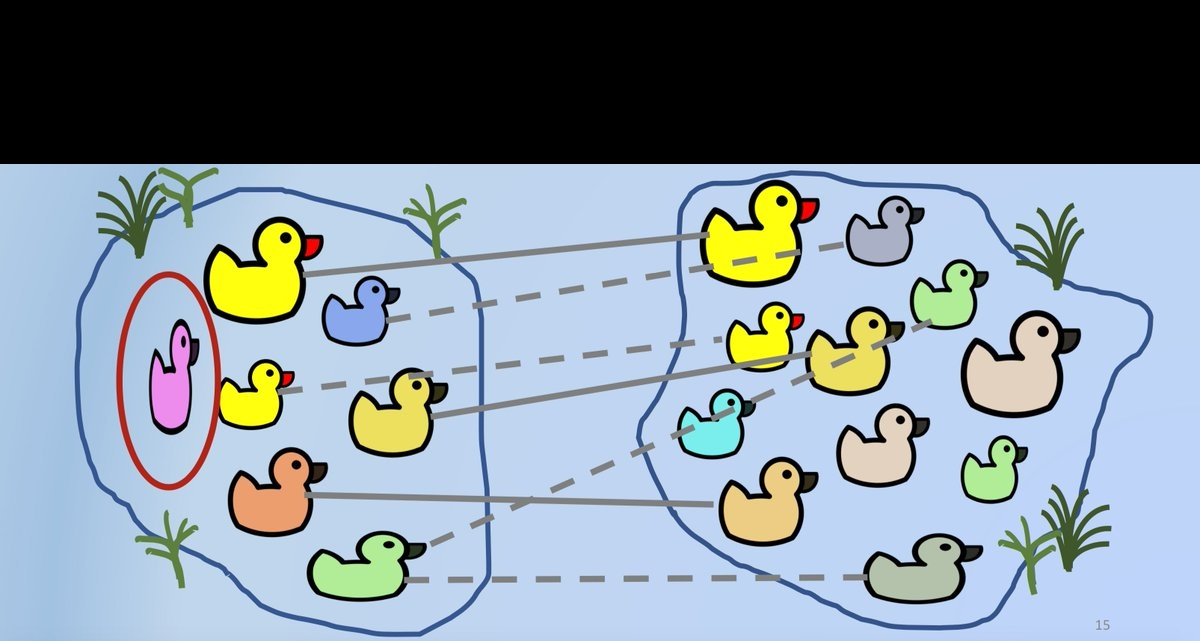
\includegraphics[trim = 0cm 0cm 0cm 6cm, clip, width=0.5\textwidth]{./IMG/PSM1}
\\
\medskip
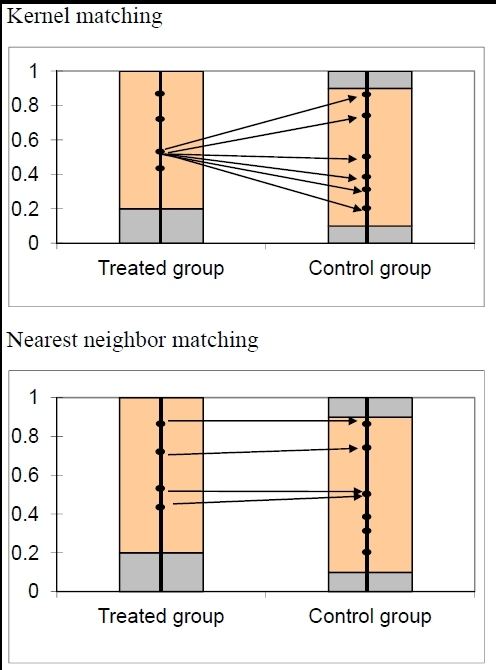
\includegraphics[trim = 0.1cm 0.15cm 0cm 0.15cm, clip, width=0.3\textwidth]{./IMG/PSM2}
\end{frame}
%---------------------------------
\begin{frame}{PSM: Assumptions and features}
\begin{itemize}
    \item \emph{Unconfoundedness:} assignment to the treatment is independent of the potential outcomes given a set of observed covariates.
    \item \emph{Common Support} or overlap condition, meaning that individuals with the same characteristics have a positive probability of being both in the treatment and control group.
    \item \emph{Large sample sizes:} PSM often requires large sample sizes because matching may not be possible if the overlap between treatment and control groups is not sufficient.
    \bigskip
    \item \emph{Matching}: PSM involves pairing treated and untreated subjects who have similar propensity scores.
    \item \emph{Propensity score} is a balancing score. Conditional on the propensity score, distribution of observed baseline covariates will be similar between treated and untreated subjects.
\end{itemize}
\end{frame}
%---------------------------------
\begin{frame}{PSM: Main steps}
\begin{enumerate}
    \item Collect data, identify that PSM is viable and appropriate
        \begin{itemize}
            \item Assumptions
        \end{itemize}
    \item Calculate propensity scores
        \begin{itemize}
            \item Logit/probit with exposure (treatment) as dependent variable
            \item Include all predictors of the exposure and none of effects of the exposure. We may include confounders and interaction variables.
        \end{itemize}
    \item Match subjects on the propensity scores
        \begin{itemize}
            \item 1-to-1 matching, 1-to-n matching
            \item Nearest neighbor, Caliper (type of NN), Kernel, Radius, etc.
        \end{itemize}
    \item Assess quality of the matching\\
        \begin{itemize}
            \item Substantial overlap (covariates) between treated \& control groups
            \item Use diagnostic metrics (e.g. standardized difference)
        \end{itemize}
    \item Analyze the propensity-matched data
        \begin{itemize}
            \item Multiple regression models (use treatment as model variable) 
            \item DiD on matched data, survival analysis, etc.
        \end{itemize}
\end{enumerate}
\end{frame}
%---------------------------------
% https://www.publichealth.columbia.edu/research/population-health-methods/propensity-score-analysis 
% 
% https://journals.lww.com/anesthesia-analgesia/fulltext/2018/10000/five_steps_to_successfully_implement_and_evaluate.37.aspx
%---------------------------------


\section{Regression discontinuity design}
\begin{frame}{Regression discontinuity design}
    Violates common support assumption
\end{frame}
%---------------------------------
\subsection{Regression discontinuity design}
\begin{frame}{Regression discontinuity design}
\begin{figure}
    \centering
    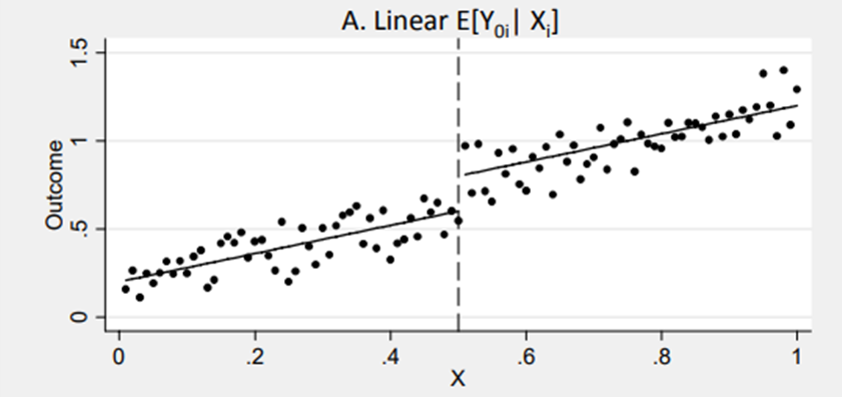
\includegraphics[width=0.6\textwidth]{./IMG/RDD1.png} 
    \caption*{RDD: treatment effect visualization example,\\ linear, common slope.}
    \label{fig:my_label}
\end{figure}    
  
    
\end{frame}
%---------------------------------
\begin{frame}{Regression discontinuity design -- potential problems}
\begin{itemize}
    \item[I.a] Misspecification of the model/functional form, which is used to estimate treatment effect.\\
    \bigskip
    Linearity is often the default approach (assumption) in regression models. However, this may not reflect real DGP. For proper treatment effect estimation, model should be accurately formulated. If appropriate, use quadratic forms, higher polynomials or LOESS (locally estimated scatterplot smoothing).
\end{itemize}
\begin{figure}
    \centering
    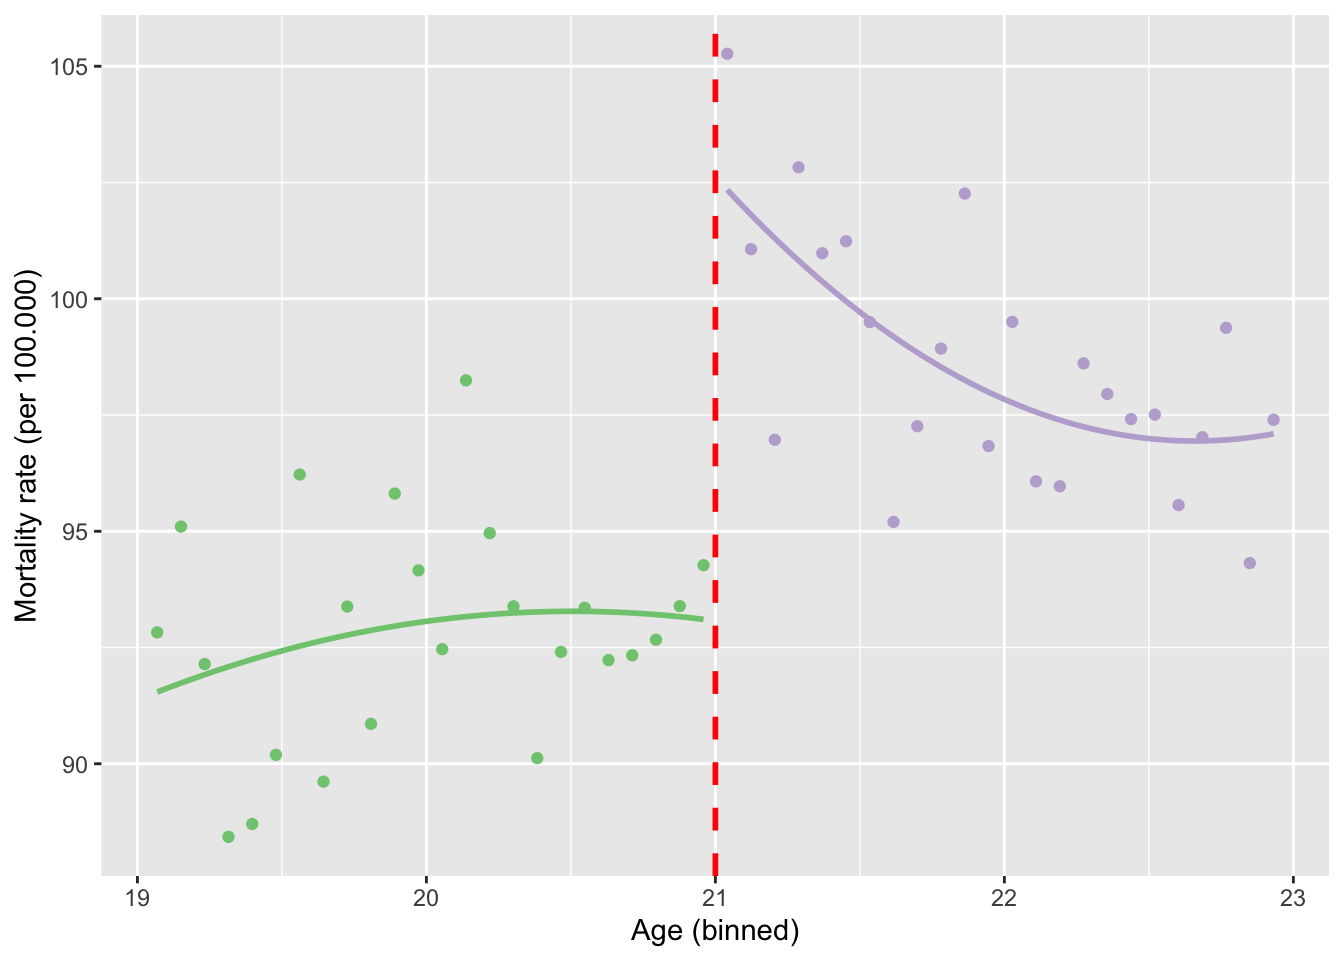
\includegraphics[width=0.55\textwidth]{./IMG/RDD2.png} 
    \caption*{True outcome function can be non-linear.} \label{fig:my_label1}
\end{figure}    
\end{frame}
%---------------------------------
\begin{frame}{Regression discontinuity design -- potential problems}
\begin{itemize}
    \item[I.b] Misspecification of the model/functional form, which is used to estimate treatment effect.\\ 
    \bigskip
    Possibly, once a nonlinear relationship is modelled correctly, discontinuity disappears as it was caused by a misspecification in the functional form. In the plot below, the correct relationship is specified by a curve. If we use a linear relationship, we might observe a (spurious) discontinuity.
\end{itemize}
\begin{figure}
    \centering
    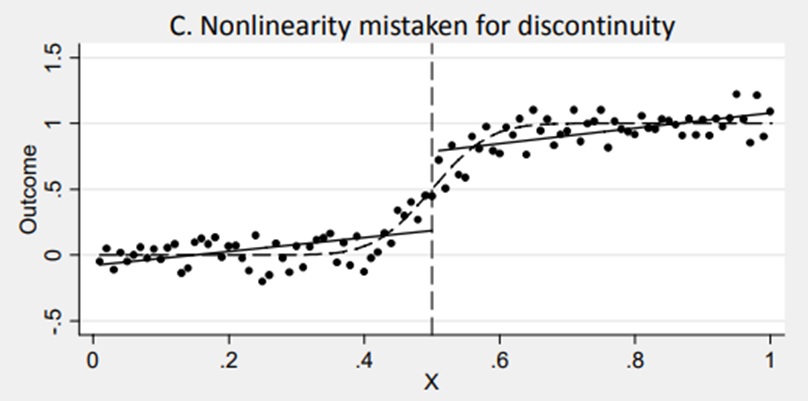
\includegraphics[width=0.55\textwidth]{./IMG/RDD3.png}
    \caption*{``Discontinuity'' caused by functional misspecification.} \label{fig:my_label2}
\end{figure}    
\end{frame}
%---------------------------------
\begin{frame}{Regression discontinuity design -- potential problems}
\begin{itemize}
    \item[II.] Diffusion of the treatment.\\ \bigskip \small
    
    RDD assumes that all individuals below (or above) the cutoff point received the treatment and vice versa.\\ \smallskip
    In reality, the treatment and the control groups can be ``contaminated''. Say, despite mandatory attendance policy (below a given grade average), some students do not attend classes. Alternatively, individuals below (or above) the cutoff might be \textit{allowed} to attend special classes or programs. \\ \medskip

    \textbf{RDD fuzzy design}: cut off is probabilistic. Methodology \& solutions:\\

    \begin{itemize}
        \item Acknowledge possible issues, but still run RDD model comparing eligible vs ineligible individuals.
        \item Use eligibility as an instrument (IV). First estimate treatment probability, then use RDD to estimate the treatment on the treated.
        \item \textcolor{blue}{\underline{\href{https://onlinelibrary.wiley.com/doi/10.1111/1468-2354.t01-1-00055}{Methodology details provided by: van der Klaauw, 2003}}}
    \end{itemize}


\end{itemize}
\end{frame}
%---------------------------------

\subsection{Propensity score matching}
\begin{frame}{Propensity score matching}
    Greene 19.6.2
\end{frame}
%---------------------------------





%---------------------------------
\begin{frame}{Treatment effects - additional literature}
\textbf{Treatment effects}\\
\medskip
For detailed \& technical discussion, see:\\
\medskip
\begin{itemize}
\item[1.] Greene: Econometric analysis, chapter 19.6
\medskip
\item[2.] Angrist, Pischke: Mostly Harmless Econometrics
\medskip
\item[3.] Cameron, Trivendi: Microeconometrics, Methods and Applications, chapter 25
\medskip
\item[4.] Wooldridge: Econometric analysis of C-S and panel data, chapter 21 Estimating Average Treatment Effects
\end{itemize}
\end{frame}
%---------------------------------
%---------------------------------------------------------------------
\end{document}